\documentclass{article}

% if you need to pass options to natbib, use, e.g.:
%     \PassOptionsToPackage{numbers, compress}{natbib}
% before loading neurips_2018

% ready for submission
% \usepackage{neurips_2018}

% to compile a preprint version, e.g., for submission to arXiv, add add the
% [preprint] option:
     \usepackage[final]{neurips_2018}

% to compile a camera-ready version, add the [final] option, e.g.:
%     \usepackage[final]{neurips_2018}

% to avoid loading the natbib package, add option nonatbib:
%     \usepackage[nonatbib]{neurips_2018}

\usepackage[utf8]{inputenc} % allow utf-8 input
\usepackage[T1]{fontenc}    % use 8-bit T1 fonts
\usepackage{hyperref}       % hyperlinks
\usepackage{url}            % simple URL typesetting
\usepackage{booktabs}       % professional-quality tables
\usepackage{amsfonts}       % blackboard math symbols
\usepackage{nicefrac}       % compact symbols for 1/2, etc.
\usepackage{microtype}      % microtypography
\usepackage{float}
\usepackage{graphicx}
\usepackage{amsmath,amssymb} 
\usepackage{physics}
\usepackage{longtable}
\usepackage{tabularx}
\usepackage{listings}
\usepackage{color}
 
\definecolor{codegreen}{rgb}{0,0.6,0}
\definecolor{codegray}{rgb}{0.5,0.5,0.5}
\definecolor{codepurple}{rgb}{0.58,0,0.82}
\definecolor{backcolour}{rgb}{0.40,0.40,0.40}
 
\lstdefinestyle{mystyle}{
    %backgroundcolor=\color{backcolour},   
    commentstyle=\color{backcolour},
    keywordstyle=\color{codegreen},
    numberstyle=\tiny\color{codegray},
    stringstyle=\color{codepurple},
    basicstyle=\footnotesize,
    breakatwhitespace=false,         
    breaklines=true,                 
    captionpos=b,                    
    keepspaces=true,                 
    numbers=left,                    
    numbersep=5pt,                  
    showspaces=false,                
    showstringspaces=false,
    showtabs=false,                  
    tabsize=2
}



\lstset{style=mystyle}




\title{Deep Neural Networks - A bird's-eye view}

% The \author macro works with any number of authors. There are two commands
% used to separate the names and addresses of multiple authors: \And and \AND.
%
% Using \And between authors leaves it to LaTeX to determine where to break the
% lines. Using \AND forces a line break at that point. So, if LaTeX puts 3 of 4
% authors names on the first line, and the last on the second line, try using
% \AND instead of \And before the third author name.

\author{%
  Jose Luis Silva\thanks{https://jseluis.github.io/} \\
  Department of Physics and Astronomy\\
  Uppsala University\\
  Uppsala, SE 751 20 \\
  \texttt{jose.silva@physics.uu.se} \\
  % Affiliation \\
  % Address \\
  % \texttt{email} \\
  % \AND
  % Coauthor \\
  % Affiliation \\
  % Address \\
  % \texttt{email} \\
  % \And
  % Coauthor \\
  % Affiliation \\
  % Address \\
  % \texttt{email} \\
  % \And
  % Coauthor \\
  % Affiliation \\
  % Address \\
  % \texttt{email} \\
}
\makeatletter
\renewcommand{\@noticestring}{}
\makeatother
\begin{document}
% \nipsfinalcopy is no longer used

\maketitle

\begin{abstract}
******** to be updated ***********\\
In this report we will explore the logistic regression method for binary classification. As part of the assignments, I will also provide details about the implementations in Python. This means an explanatory bird's-eye view of how to optimize parameters of the model using gradient descent method, Binary Cross-Entropy loss function and cost function derivatives. Additionally, we will use the biopsy breast cancer dataset to deploy the model and evaluate the accuracy to predict if a certain biopsy is "benign" or "malignant".
\end{abstract}

\section{Introduction}
******** to be updated ***********\\
In binary classification tasks, our main interest is to determine optimized parameters of a model that can efficiently predict the probability mass function $p(y = 1 | x)$ of an event $y \in \{0,1\}$ given x on a specific interval $[0,1]$.  In our case, we want to find a set parameters using the logistic regression model to predict the probability vector $p_i=P(y_i = 1 | x_i)$ for a data set with $i=\{1, 2,..., n-1, n\}$ inputs vectors ${\bold{x}_i }$ and $y_i$ outputs where $y_i \in \{0,1\}$, $\bold{x}_i  = [ x_{i1},x_{i2},..,x_{i(p-1)},x_{ip}]^T$ and $p=\{1, 2,..., m-1, m\}$ features. For each input vector $\bold{x}_i $, logistic regression model can be summarized as computing the following set of linear combinations:
\begin{eqnarray}
z_1&=&\sum_{j=1}^{p} w_{j} x_1j +b \nonumber \\
z_2&=&\sum_{j=1}^{p} w_{j} x_2j +b \nonumber \\
\vdots \nonumber \\
z_n&=&\sum_{j=1}^{p} w_{j} x_nj +b = \bold{w}^T \bold{x}_i + b \nonumber \\
\end{eqnarray}
where $n$ is the number of input vectors, $p$ the number of features in each input vector, $b$ represents the  offset parameter and $\bold{w}=[w_1,w_2,...,w_p]^T$ the weights. As a first step we can generate a set of normalized random values to initialize the weights and the offset b. This procedure allows the computation of the probability that each input vector $\bold{x}_i$ belongs to certain class $y_i =\{1,0\}$. Hence, we can apply the activation function(sigmoid) over $\bold{z}_i$, such that:
\begin{eqnarray}
p_i=& \sigma(z_i) = \left[1+\exp(-\sum_{j=1}^{p} w_{j} x_ij +b )\right]^{-1} \nonumber \\
\end{eqnarray}
This procedure is followed by an optimization of the model through the maximization of the likelihood for a given set of parameters. We use the cross-entropy loss $L(p_i,y_i)$ function for each input vector and take an average over the whole data set to estimate an initial cost function $J(p_i,y_i)$, where:
\begin{eqnarray}
J &=& \frac{1}{n} \sum_{i=1}^{n} L(p_i,y_i) \\
L(p_i,y_i)&=& -y_i \ln(p_i) - (1-y_i) \ln(1-p_i)
\end{eqnarray}
However, the parameters of the model are optimized through a stochastic gradient descent method, which makes use of the gradient of the cost function with respect to the parameters of the model. We need to update the weights $w_i$ and the offset b for , such that:
\begin{eqnarray}
w_1^{l}&=&w_{1}^{(l-1)} - \alpha \frac{\partial{J}}{\partial{w_1}} \nonumber \\
w_2^{l}&=&w_{2}^{(l-1)} - \alpha \frac{\partial{J}}{\partial{w_2}} \nonumber \\
\vdots \nonumber \\
w_n^{l}&=&w_{n}^{(l-1)} - \alpha \frac{\partial{J}}{\partial{w_n}} \\
b^{l}&=&b^{(l-1)} - \alpha \frac{\partial{J}}{\partial{b}}
%%J &=& \frac{1}{n} \sum_{i=1}^{n} L(p_i,y_i) \\
%L(p_i,y_i)&=& -y_i \ln(p_i) - (1-y_i) \ln(1-p_i)
\end{eqnarray}
where (l-1) represents parameter from the previous iteration and $\alpha$ is responsible to modulate the learning rate. We need to determine the expressions for $\frac{\partial{J}}{\partial{w_n}}$ and $\frac{\partial{J}}{\partial{b}}$ as a function of the input data and parameter of the model. By using the chain rule, we can derive both equations as follows:
\begin{eqnarray}
&&\frac{\partial{J}}{\partial{w_j}} = \frac{\partial{J}}{\partial{z_i}} \frac{\partial{z_i}}{\partial{w_j}}   =  \frac{\partial{J}}{\partial{z_i}} \left( \frac{\partial}{\partial{w_j}}\right)\left(\sum_{i=1}^{p}w_j x_{ij} + b\right) = \left(\frac{\partial{J}}{\partial{z_i}}\right) x_{ij}
\\
&&\frac{\partial{J}}{\partial{b}} = \frac{\partial{J}}{\partial{z_i}} \frac{\partial{z_i}}{\partial{b}}   =  \frac{\partial{J}}{\partial{z_i}} \left( \frac{\partial}{\partial{b}}\right)\left(\sum_{i=1}^{p}w_j x_{ij} + b\right) = \left(\frac{\partial{J}}{\partial{z_i}}\right)
%%= \frac{1}{n}\sum_{i=1}^{n} \frac{\partial{L_i}}{\partial{w_j}}  = \frac{1}{n}\sum_{i=1}^{n} \frac{\partial{L_i}}{\partial{w_j}}\frac{\partial{L_i}}{\partial{w_j}}\frac{\partial{L_i}}{\partial{w_j}}
\end{eqnarray}
From equation (7) and (8), $\frac{\partial{J}}{\partial{z_i}} $ can be estimated using the derivation chain rule with the partial derivative of the cross-entropy loss function in respect to $p_i$, as follows:
\begin{eqnarray}
&&\frac{\partial{J}}{\partial{z_i}} =  \frac{1}{n}\sum_{i=1}^{n} \frac{\partial{L_i}}{\partial{z_i}}  = \frac{1}{n}\sum_{i=1}^{n} \frac{\partial{L_i}}{\partial{p_i}}\frac{\partial{p_i}}{\partial{z_i}} 
\end{eqnarray}
such that:
\begin{eqnarray}
&&\frac{\partial{p_i}}{\partial{z_i}} = \left(\frac{\partial{}}{\partial{z_i}}\right)  \left[1+\exp(-\sum_{j=1}^{p} w_{j} x_ij +b )\right]^{-1} = e^{-z_i}(1+e^{-z_i})^{-2} 
%%\\=
\end{eqnarray}
and since:
\begin{eqnarray}
p_i = (1+e^{-z_i}) ^{-1} \rightarrow e^{-z_i} = p^{-1} -1 = \frac{(1-p_i)}{p_i}
\end{eqnarray}
equation (10) becomes:
\begin{eqnarray}
&&\frac{\partial{p_i}}{\partial{z_i}} =  \frac{(1-p_i)(1+e^{-z_i})^{-2} }{p_i}=p_i(1-p_i)
\end{eqnarray}
The first partial derivative from equation (9) becomes:
\begin{eqnarray}
&&\frac{\partial{L_i}}{\partial{p_i}} =  -\frac{y_i}{p_i} + \frac{(1-y_i)}{(1-p_i)}
\end{eqnarray}
therefore:
\begin{eqnarray}
&&\frac{\partial{J}}{\partial{z_i}} =  \frac{1}{n}\sum_{i=1}^{n} \left[-\frac{y_i}{p_i} + \frac{(1-y_i)}{(1-p_i)} \right] \left[  \frac{(1-p_i)}{p_i} \right] = \frac{1}{n}\sum_{i=1}^{n} [ -y_i(1-p_i) + p_i(1-y_i)] \nonumber \\ &&=  \frac{1}{n}\sum_{i=1}^{n}(p_i-y_i) \nonumber \\
\end{eqnarray}

In order to update the parameters of the model, the following set of recurrent formulas were implemented in python:
\begin{eqnarray}
w_1^{l}&=&w_{1}^{(l-1)} -  \frac{\alpha}{n}\sum_{i=1}^{n}(p_i-y_i)x_{1j}\nonumber \\
w_2^{l}&=&w_{2}^{(l-1)} - \alpha   \frac{\alpha}{n}\sum_{i=1}^{n}(p_i-y_i)x_{2j} \nonumber \\
\vdots \nonumber \\
w_n^{l}&=&w_{n}^{(l-1)} - \frac{\alpha}{n}\sum_{i=1}^{n}(p_i-y_i)x_{nj} \\
b^{l}&=&b^{(l-1)} -  \frac{\alpha}{n}\sum_{i=1}^{n}(p_i-y_i)
%%J &=& \frac{1}{n} \sum_{i=1}^{n} L(p_i,y_i) \\
%L(p_i,y_i)&=& -y_i \ln(p_i) - (1-y_i) \ln(1-p_i)
\end{eqnarray}

For the exercise 1.3, the logistic regression model that can be trained with stochastic gradient descent was implemented in Python using Numpy library for vectorization and faster operations. I have created following trained data set:  $n=6$ input vectors with two features $x_i=[x_1,x_2]$ and outputs $y_i={1,0}$ where $y_i=1$ if $x_1=x_2$ or $x_1>x_2$ and $y_i = 0$ if $x_2>x_1$: 

\begin{eqnarray}
x\_train &=& np.array([[1,1],[3,4],[5,5],[7,7],[1,4],[4,4]])  \\
x\_test &=& np.array([[3,3],[3,10],[1,5],[12,12],[1,0],[10,100]]) \\
y\_train &=& np.array([1,0,1,1,0,1]) \\
y\_test &=& np.array([1,0,0,1,1,0]) \\
\end{eqnarray}

An initialization function was responsible for starting a set of parameter such as a fixed learning rate of 0.5 and break of the self-consistent loops based on values of the cost function which should be lower than 0.001 (convergence break). The training was performed for 18151 steps until the break of the while loop due to convergence. The set of equations for the sigmoid activation function, cost function and proper deduced gradients to update the parameters of the model during every iteration were implemented as functions in Python and called inside the while loop. The accuracy for the predictions based on the optimized parameters was 100$\%$ and consequently the confusion matrix matched the number of True Positives and True Negatives of the test data set. The code is well explained in the appendix session.

	For the exercise 1.4, I have used the same python functions and part of the previous implementation with some changes in order to predict the biopsy as malignant or benign in the test data set using the optimized model. First we initialized the variables and used a learning rate of 0,8. We reshaped  Y for train and test to (300,) and (383,) respectively. Additionally I have applied a normalization of $X_{train}$ and $X_{test}$ dividing by the maximum value of the features. The functions to estimate the probabilities, cost function and gradients are optimized for any $X_{train}$ and $X_{train}$ shape. I have included arrays to append the cost function during the optimization of the parameters for both training and test data set in order to plot the cost function x number of iterations. We optimized the parameters with 4577 iterations considering a threshold $min_{cost}$ of 0.61. The cost function decays very fast as a function of the iteration, as shown in the Figure \ref{fig:cancer}.

\begin{figure}[H]
    \centering
    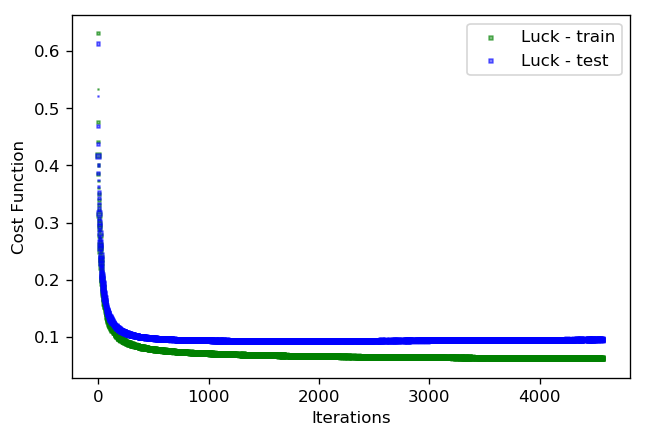
\includegraphics[width=1\linewidth]{cost_function}
    \caption{Cost function x Iteration - Blue = Test data set , Green = Train data set}
    \label{fig:cancer}
\end{figure}

As expected, the the cost function is lower for the training data set (green color) as compared to the testing data set. The accuracy of the model on the training and test data set was 0.97 and 0.96, respectively. The confusion matrix for the training and test data set showed a very low number of False Negatives with 5 missed predictions as malignant in both cases.  We conclude that the logistic regression model optimized with stochastic gradient descent is very accurate for binary classification predictions in this particular data set.

\newpage

\section{Appendix}
Exercise 1.3
\begin{lstlisting}[language=Python]
import numpy as np
import matplotlib.pyplot as plt

#		The shape of x_train and x_test is (6, 2) and  y_test and y_train is (6,). Each vector has two features x1,x2 that belongs to a class y=0 or y=1. If x1=x2 or #  x1>x2 then y = 0 otherwise y=0.

x_train = np.array([[1,1],[3,4],[5,5],[7,7],[1,4],[4,4]]) 
y_train = np.array([1,0,1,1,0,1])
x_test = np.array([[3,3],[3,10],[1,5],[12,12],[1,0],[10,100]])
y_test = np.array([1,0,0,1,1,0])

#		Initialization of the parameters through initialize() function. The weights were chosen randomly using a normal distribution with gaussians. The transpose of x_train is initialized for future matrix operations. The initial offset b = 0 and min_cost controls the number of iterations to minimize the cost function by breaking the self-consistent loop when the cost function is lower than 0.001

def initialize(x_train,y_train):
    w = np.random.random([x_train.shape[1]])
    n = x_train.shape[0]
    x = np.transpose(x_train)
    b = 0
    alpha = -0.5
    min_cost = 0.001 # Control variable to stop the minimization of the cost function
    return w,x,n,b,alpha,min_cost
    
#		Definition of activation function sigma(z) based on the sigmoid. the function needs to be called by defining the type of activation. i.e sigma(z,activation='sigmoid'). This is important if we explore possible different activation functions in the next assignments.

def sigma(z_i,activation=False):
    if(activation==False):
        return print('Please choose an activation function')
    elif(activation=='sigmoid'):
        sig = 1/(1+np.exp(-z_i))
        return sig

#		This function calculates the cross-entropy loss function and the cost function. Instead of using for-loops element-wise operations are performed with arrays. You need to define which type of loss function to use: cost_function(y_train,p_i,loss_function='cross_entropy')

def cost_function(y_i,p_i,loss_function=False):
    if(loss_function==False):
        return print('Please choose a loss function')
    elif(loss_function=='cross_entropy'):
        n = y_i.shape[0]
        loss_calc = -(y_i*np.log(p_i)+ (1-y_i)*(np.log(1-p_i)))
        cost_calc = (1/n)*np.sum(loss_calc)
        return loss_calc,cost_calc
        
#		This function calculates the gradients and performs matrix operations to estimate the partial derivatives. dLdb represents the derivative of the loss function with respect to the offset parameter b. dJdb = derivative of the cost function with respect to b and dJdw = derivative of the cost function with respect to a specific j-th weight. Numpy library was used for vectorization and to perform element-wise operations instead of for loops.  

def grad(p_in,y_in,x_in): # input p_in = array of probability, y_in = array of classes, x_in = matrix array.
    n_in = y_in.shape[0]
    dLdb = p_in - y_in
    dJdb = (1/n_in)*np.sum(dLdb) # Derivative of the Cost function with respect to offset  
    dJdw = (1/n)*np.dot(dLdb,x_in) # Vectorization to facilitate the operations and automatically perform the sum.
    return dJdw,dJdb
 
# 		Initialize w=weight, x=input vectors, n= number of input vectors in the data set, alpha = learning rate, min_cost = control variable

w,x,n,b,alpha,min_cost=initialize(x_train,y_train)

# 		Calculate an initial z using matrix formulation where  x = transpose of x_train. Here we also calculate the sigmoid for each z and print the values.

z = np.dot(w,x)+b
p_i=sigma(z,activation='sigmoid')
print('z =',z,'\ny_i =',y_train,'n =',n, 'w =',w)
print('p_i = ',p_i)

#		Function call to estimate the cost function based on the cross-entropy loss function and print both the cost function and the loss function. l = loss function, j = cost function

l,j= cost_function(y_train,p_i,loss_function='cross_entropy') 
print('Cost Function =',j,'\nLoss Function vector =',l)

#		Function call to estimate the gradients dw = dJdw and db = dJdb. These values are used to update the parameter of the model.

dw,db= grad(p_i,y_train,x_train)
print(dw,db)

#		First update of the weight and offset parameters.

w += alpha*dw
b += alpha*db
print('w =',w,'\n b =',b)

#		Definition of a counter and threshold of min_cost = 0.001 for convergence. This means that the parameters of the model are optimized. All the previous operations are performed inside the loop until the break of the self-consistent while-loop.

counter = 0
while(j>min_cost):
    z = np.dot(w,x)+b
    counter+=1
    p_i=sigma(z,activation='sigmoid')
    l,j= cost_function(y_train,p_i,loss_function='cross_entropy')
    print('Cost Function =',j,'\n')
    dw,db = grad(p_i,y_train,x_train)
    w +=alpha*dw
    b +=alpha*db
print('Number of iterations = ',counter)

#		In order to test the optimization over the training data set, prediction_train checks each probability found with the new parameters and approximates to 1 if p_i > 0.5 and 0 otherwise.

prediction_train = np.where(p_i>0.5,1,0)
print(prediction_train)

#		Calculate the prediction over the test dataset 
z_test = np.dot(w,np.transpose(x_test))+b
p_i_test=sigma(z_test,activation='sigmoid') # probability using optimized parameters
prediction_test = np.where(p_i_test>0.5,1,0)  # threshold of 0.5 to approximate y values
print(prediction_test)
np.mean(prediction_test == y_test) # Calculate the accuracy
print(pd.crosstab(prediction_test, y_test)) # Check the confusion matrix
\end{lstlisting}

Exercise 1.4
\begin{lstlisting}[language=Python]
# Import Numpy, Matplotlib and Pandas library
import numpy as np
import matplotlib.pyplot as plt
import pandas as pd

#		Function to initialize the biopsy data set.

def load_biopsy():
    # import data
    biopsy = pd.read_csv('biopsy.csv', na_values='?', 
                         dtype={'ID': str}).dropna().reset_index()
    
    # Split in training and test data
    trainI = np.random.choice(biopsy.shape[0], size=300, replace=False)    
    trainIndex=biopsy.index.isin(trainI)    
    train=biopsy.iloc[trainIndex] # training set
    test=biopsy.iloc[~trainIndex] # test set    
    
    # Extract relevant data features
    X_train = train[['V1','V2','V3','V4','V5','V6','V7','V8','V9']].values
    X_test = test[['V1','V2','V3','V4','V5','V6','V7','V8','V9']].values    
    Y_train=(train['class']=='malignant').astype(int).values.reshape((-1,1))
    Y_test=(test['class']=='malignant').astype(int).values.reshape((-1,1))
    
    return X_train, Y_train, X_test, Y_test

# Initialization of the parameters through initialize() function. 
# The weights were chosen randomly using a normal distribution with gaussians.
# The transpose of x_train is initialized for future matrix operations. 
# The initial offset b = 0 and min_cost  controls the number of iterations to minimize the cost function by breaking the self-consistent loop when the cost function is lower than 0.062

def initialize(x_train,y_train):
    w = np.random.random([x_train.shape[1]])
  # w=np.array([0.39401661, 0.47478989, 0.06309985, 0.99740423, 0.33530285,0.60437357, 0.74371789, 0.3407668 , 0.81388953]) # Initial parameters generated randomly.
    n = x_train.shape[0]
    x = np.transpose(x_train)
    b = 0
    alpha = -0.8 # Learning rate of 0.8
    min_cost = 0.062
    return w,x,n,b,alpha,min_cost

# Definition of activation function sigma(z) based on the sigmoid. 
# This function needs to be called by defining the type of activation function. i.e sigma(z,activation='sigmoid'). 
# This is important if we explore possible different activation functions in the next assignments.

def sigma(z_i,activation=False):
    if(activation==False):
        return print('Please choose an activation function')
    elif(activation=='sigmoid'):
        sig = 1/(1+np.exp(-z_i))
        return sig
        
# This function calculates the cross-entropy loss function and the cost function. 
# Instead of using for-loops element-wise operations are performed with arrays. 
# You need to define which type of loss function to use: cost_function(y_train,p_i,loss_function='cross_entropy')
 
def cost_function(y_i,p_i,loss_function=False): 
    if(loss_function==False):
        return print('Please choose a loss function')
    elif(loss_function=='cross_entropy'):
        n = y_i.shape[0]
        loss_calc = -(y_i*np.log(p_i) + (1-y_i)*(np.log(1-p_i)))
        cost_calc = (1/n)*np.sum(loss_calc)
        return loss_calc,cost_calc

# This function calculates the gradients and performs matrix operations to estimate the partial derivatives. 
# dLdb represents the derivative of the loss function with respect to the offset parameter b. 
# dJdb = derivative of the cost function with respect to b and dJdw = derivative of the cost 
# function with respect to a specific j-th weight. 
# Numpy library was used for vectorization and to perform element-wise operations instead of for loops.  

def grad(p_in,y_in,x_in):
    n_in = y_in.shape[0]
    dLdb = p_in - y_in
    dJdb = (1/n_in)*np.sum(dLdb)  
    dJdw = (1/n)*np.dot(dLdb,x_in) # vector dJ/dW_j to update w_j
    return dJdw,dJdb
    
# Load biopsy data in training and testing variables
X_train, Y_train, X_test, Y_test=load_biopsy() 
# Normalization of the training data set 
X_train = X_train/np.max(X_train)  
Y_train = np.reshape(Y_train,(Y_train.shape[0],)) # Reshape of the Y_train from (300, 1) to (300,)
 # Normalization of the testing data set
X_test = X_test/np.max(X_test)
Y_test = np.reshape(Y_test,(Y_test.shape[0],)) # Reshape of the Y_train from (300, 1) to (300,)

# Initialize parameters and transpose of X_train.
w,x,n,b,alpha,min_cost=initialize(X_train,Y_train)

# Initialize vector z and the probabilities p_i with the initial parameter of the model
z = np.dot(w,x)+b
p_i=sigma(z,activation='sigmoid')

# Function call to estimate the cost function based on the cross-entropy loss function and print both the cost function and the loss function. l = loss function, j = cost function
l,j= cost_function(Y_train,p_i,loss_function='cross_entropy') # l = loss function
print('Cost Function =',j,'\nLoss Function vector =',l)
 
# Function call to estimate the gradients dw = dJdw and db = dJdb. 
# These values are used to update the parameter of the model.
dw,db= grad(p_i,Y_train,X_train) 
print(dw,db)
w += alpha*dw # update weights  gradient descent
b += alpha*db # update the offset using gradient descent
print('w =',w,'\n b =',b) # print new parameters

# Definition of a counter and threshold of min_cost for convergence. This means that the parameters of the model are optimized. All the previous operations are performed inside the loop until the break of the self-consistent while.

counter = 0 # counter the iterations
cost = [] # append cost function of the training data set in the array
iter = [];  # append iteration in the array
cost_test = []; # append cost function of the test data set in the array
while(j>min_cost):
    z = np.dot(w,x)+b
    counter+=1
    p_i=sigma(z,activation='sigmoid')
    l,j= cost_function(Y_train,p_i,loss_function='cross_entropy')
    cost.append(j)
    iter.append(counter)
    
    # calculate z, p_i and cost function based on optimized parameters for the test data set.
    z_test = np.dot(w,np.transpose(X_test))+b 
    p_i_test=sigma(z_test,activation='sigmoid')
    l_test,j_test= cost_function(Y_test,p_i_test,loss_function='cross_entropy')
    cost_test.append(j_test)
    
    print('Cost Function =',j,'\n')
    dw,db = grad(p_i,Y_train,X_train)
    w +=alpha*dw
    b +=alpha*db
print('Number of iterations = ',counter)

prediction_train = np.where(p_i>0.5,1,0)

np.mean(prediction_train == Y_train) # Accuracy of 0.98 on training data set

print(pd.crosstab(prediction_train, Y_train))  # Generate the confusion matrix

# generate z and probabilities based on the optimized parameters
z_test = np.dot(w,np.transpose(X_test))+b 
p_i_test=sigma(z_test,activation='sigmoid')
prediction_test = np.where(p_i_test>0.5,1,0)

# Predict the acurracy -  0.9660574412532638 on the test data set
np.mean(prediction_test == Y_test) 

print(pd.crosstab(prediction_test, Y_test)) # Generate the confussion matrix for further analysis

# Plot the Cost Function x Iteration during the optimization for the training and test data set

plt.figure(dpi = 120)
s = np.random.rand(*x.shape)*10
plt.scatter(iter,cost,s,c="g", marker="s", alpha=0.5,label="Luck - train")
plt.scatter(iter,cost_test,s,c="b", marker="s", alpha=0.5,label="Luck - test")
plt.xlabel("Iterations")
plt.ylabel("Cost Function")
plt.legend(loc='upper right')
plt.show()

\end{lstlisting}

\section{References}
******** to be updated ***********

\end{document}
